
% please consider following Prof. Rohit's guidelines for running example

% below is just a suggestion, please adapt and continue.

% we must not present the solution below! Just illustrate the problem

% Context and Explanation of the example
To motivate the addressed research problem, a simplified example of a mission execution by entities is presented. Figure~\ref{fig:example} illustrates a reconnaissance mission where a team of four UAVs is interacting in a network configuration with a central coordinator (shown in Figure~\ref{fig:example}(a)), which is responsible only for providing instructions to its subordinates. These interactions and network topology establish the Coordinated C2 approach~\citep{FRANCE2014}. The coordinator, depicted with a dashed square around it, guides the other team members to complete mission tasks. These tasks require different types of sensors for obtaining aerial images of particular points of interest, represented by red crosses.

% Highlighting the problem
The mission has some inherent risks that may lead to a change in the conditions of execution. In this example, one member of the team, marked with a dashed circle (Figure~\ref{fig:example}(b)), dropped due to some environmental change, such as an intense storm, causing damages to its motors. The loss of one entity, depicted in Figure~\ref{fig:example}(b), can potentially decrease the effectiveness and quality of the mission execution. So, a new plan is required, considering task \textit{id 0} originally assigned to the dropped drone. Otherwise, there would be a lack of C2 agility. The absence of a system strategy to maintain or increase C2 agility may compromise the amount of completed tasks at the end of execution. 


\begin{figure}[!htbp]
	\centering
	\begin{subfigure}[t]{.45\textwidth}
	\centering
	    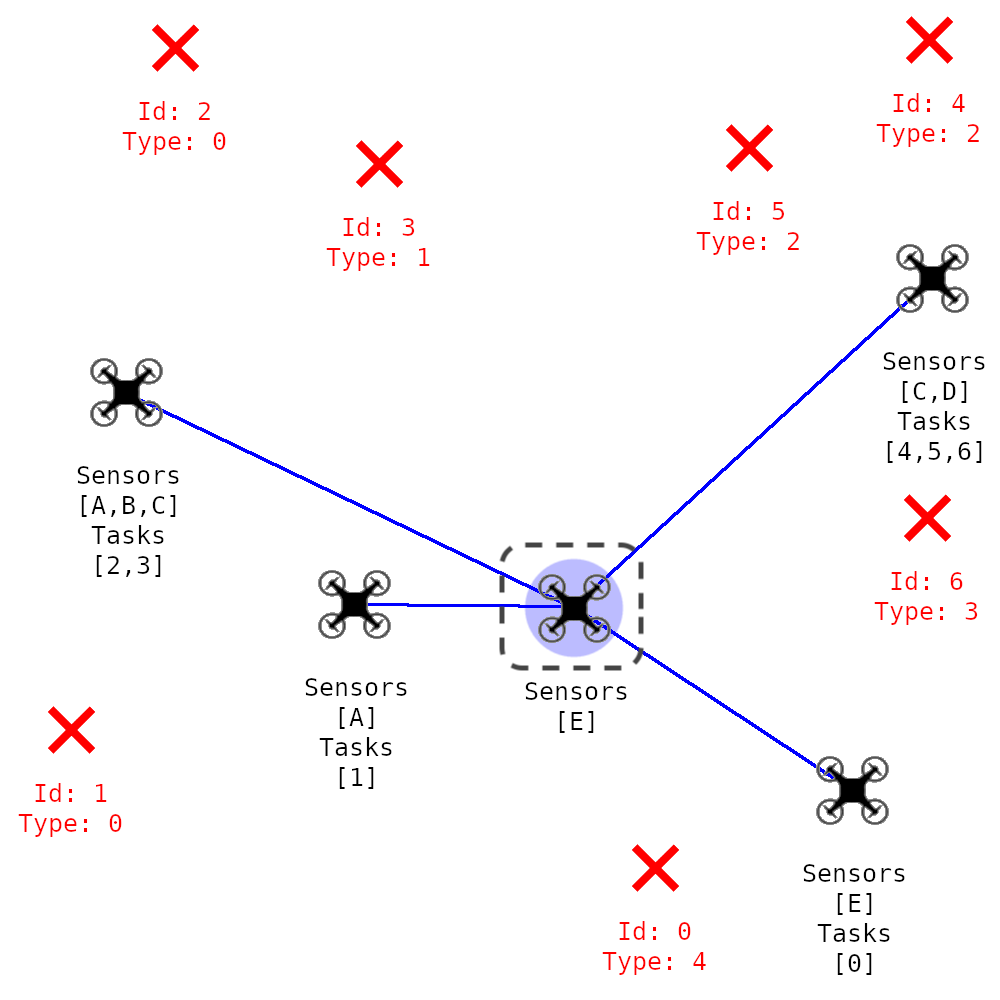
\includegraphics[width=0.95\linewidth]{img/C2Drones1-V4-dashed.png}
	    \caption{Coordinator (dashed square)\label{fig:example-a}}
	\end{subfigure}
	\begin{subfigure}[t]{.45\textwidth}
	\centering
	    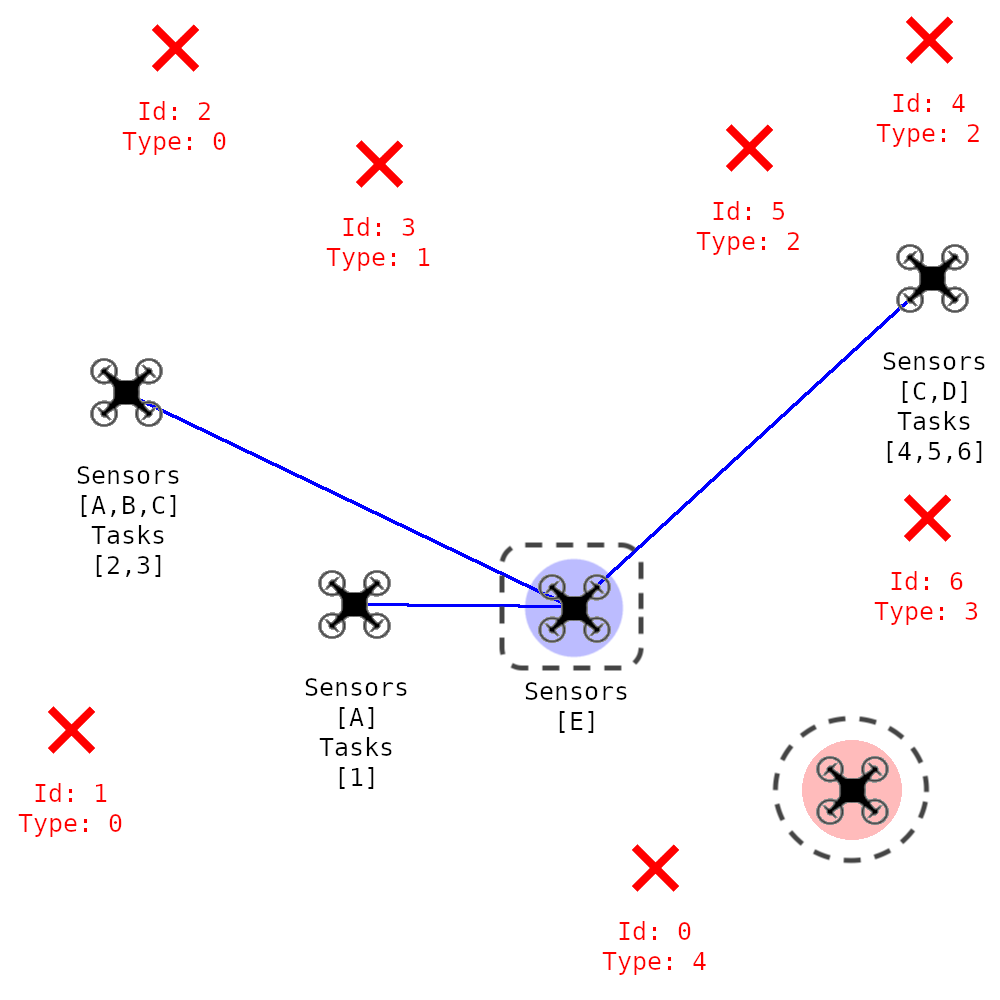
\includegraphics[width=0.95\linewidth]{img/C2Drones2-V4-dashed.png}
	    \caption{UAV dropped (dashed circle)\label{fig:example-b}}
	\end{subfigure}
	\caption{Team of entities related to a central coordinator (dashed rectangle) performing tasks at predefined locations (red crosses). A context change results in an UAV dropped (on the right, marked with a dashed circle).}
	\label{fig:example}
\end{figure}

% \begin{figure}
% \centering
% \fbox{
% \begin{minipage}{.45\textwidth}
% %\captionsetup{type=figure}
%   \centering
%   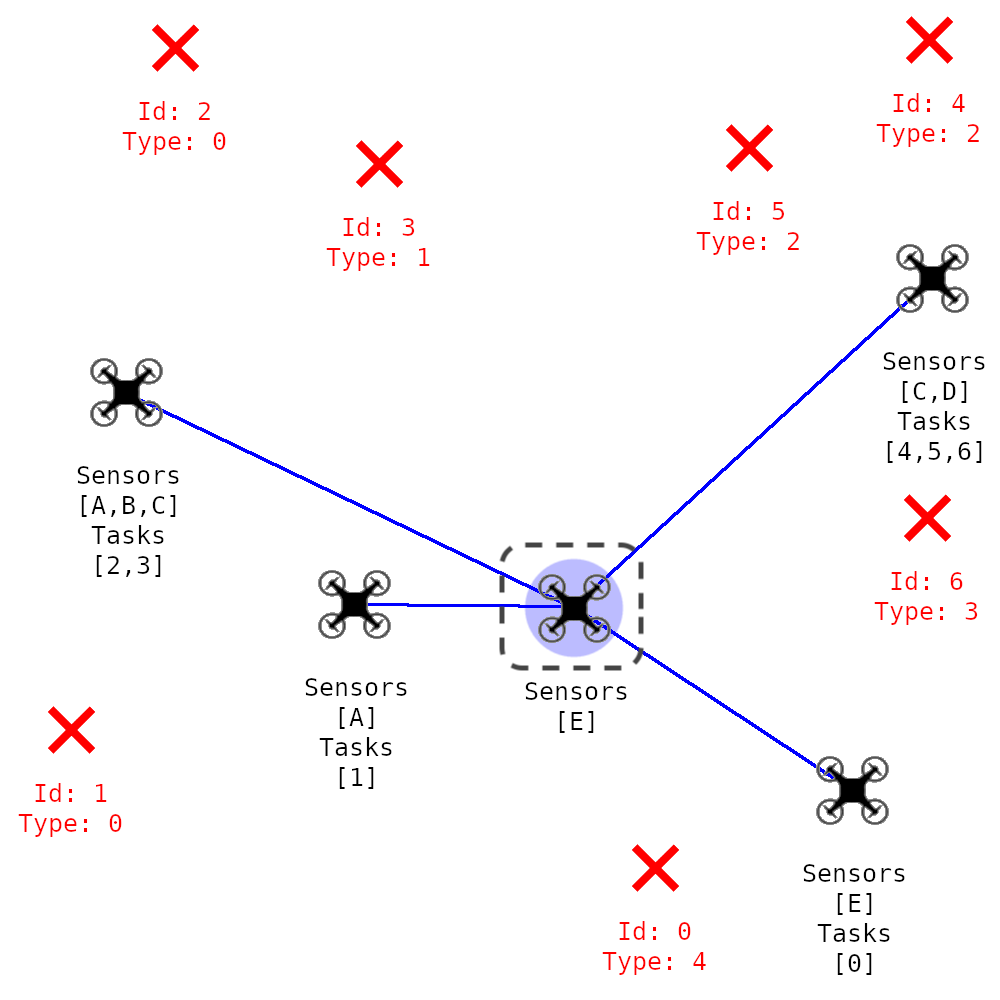
\includegraphics[width=0.95\linewidth]{img/C2Drones1-V4-dashed.png}
%   \subcaptionbox{(a) Coordinator (dashed square)\label{fig:example-a}}{}
% \end{minipage}}%
% \fbox{
% \begin{minipage}{.45\textwidth}
%   \centering
%   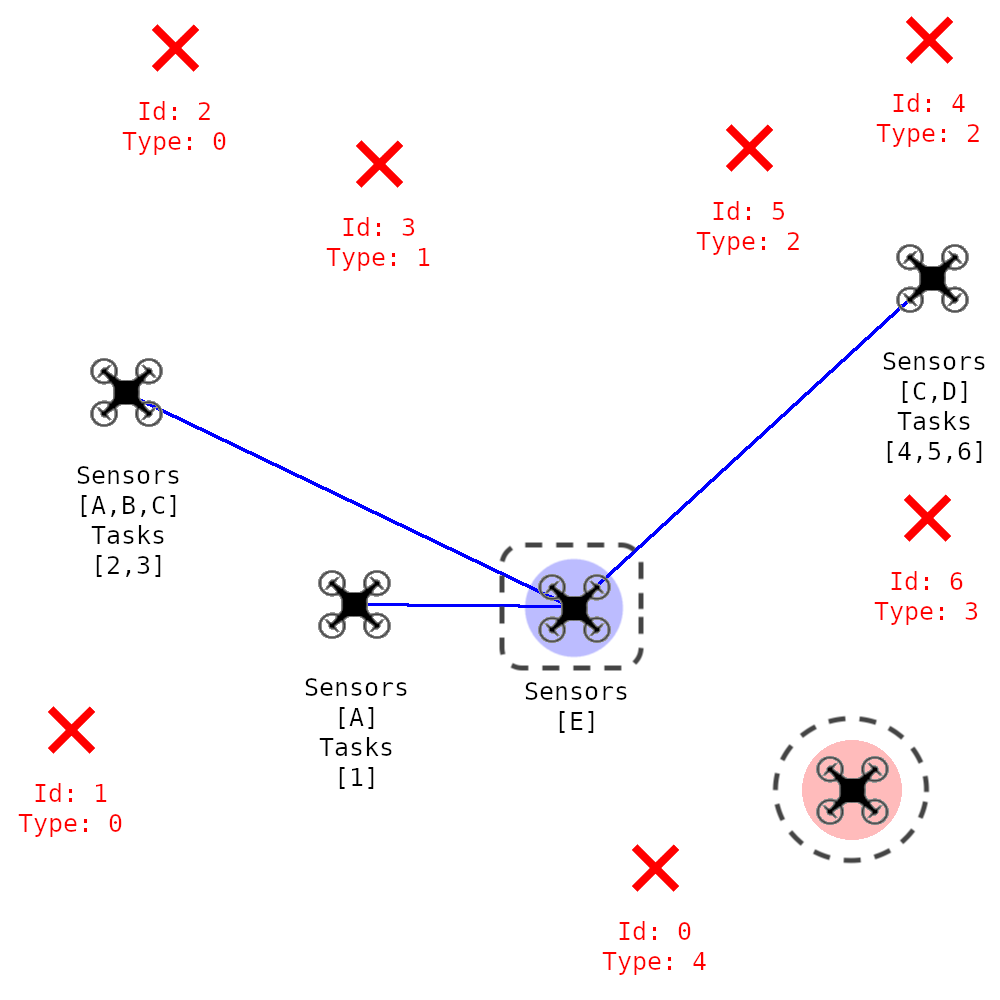
\includegraphics[width=0.95\linewidth]{img/C2Drones2-V4-dashed.png}
%   \subcaptionbox{(b) UAV dropped (dashed circle)\label{fig:example-b}}
% \end{minipage}}
% \caption{Team of entities related to a central coordinator (dashed rectangle) performing tasks at predefined locations (red crosses). A context change results in an UAV dropped (on the right, marked with a dashed circle).}
% \label{fig:example}
% \end{figure}

% Generalize the problem / Why is this not solved yet?
In general, context changes occur in the entities themselves (self) and in the environment, e.g., UAV failure, sensor damage, or weather change, and they must be considered during the mission planning.
%The self represents the entities that perform some action.
Real scenarios, where there are entities applying the available resources to accomplish a mission or to reach a goal, naturally have embedded dynamism \citep{Alberts2000, Alberts2006}. Any adaptation to the new context may decrease quality results due to an incompatibility between entities and mission, or insufficient resources to complete the mission, or even the inability to meet minimum quality acceptance level. Therefore, the C2 Agility concept introduced in Section~\ref{sec:background}, composed of C2 Approach Agility and C2 Maneuver Agility, would be compromised. This work considers a refined definition for C2 Agility as the following capability of a team in a mission:

\begin{center}
\fbox{\begin{minipage}{30em}
C2 Agility: For all tasks $t$ of a mission, it is possible to find a C2 approach $\omega$, such that a team $E$, i.e., set of members, becomes constrained to operate under $\omega$, in a way that $t$ is allocated to a member $e \in E$, and $e$ adopts  an internal configuration $c$ among its valid configurations, such that this configuration makes $e$ capable of dealing with $t$.
\end{minipage}}    
\end{center}


In other words, if there is limited C2 agility, the mission might be compromised in a dynamic context. Nevertheless, as discussed in Section~\ref{sec:relatedWork}, the state-of-art and the state-of-the-practice do not explore methodologies or strategies to provide C2 agility, especially considering context changes~\citep{Alberts2006}. 
Specifically, we consider this problem in the scope of simulation environment. This approach, which is often used to study C2 in general and in its application areas~\citep{FRANCE2014}, is relevant to explore many other scenarios such as Network Centric Warfare and telemedicine~\citep{telemedicine01, FRANCE2014, Power01}.

Even if we  represent entities’ behavior in dynamic context, modelling time constraints is outside of the scope of \X{this paper} and considered as \X{future} work. More expressive models may address such an approach, e.g., timed automata and temporal logics such as QPTL~\citep{QPTL01}. However, \X{recent works} related to C2 do not explore such a temporal aspect because of the natural complexity involved and the limitations of this field. Such works that analyze entities’ behavior in simulated and realistic \X{scenarios~\citep{FRANCE2014}}, not considering time constraints, have proven to be relevant in several domains, e.g., military.


%One possibility to avoid the problem of C2 approach agility is to change the current C2 approach, i.e., change the network configuration and leaders. Furthermore, if the team changes to an unsuitable C2 approach or is not even capable of changing its C2 approach, both cases represent a lack of C2 maneuver agility. These two types of agility compose the C2 agility concept, i.e., the entity's capability of dealing with context changes~\citep{FRANCE2014}.


%Although mission change is in the group of context changes according to \citep{Alberts10}, we are considering unchangeable set of tasks, i.e., mission does not change. We have chosen to exclude such changing of this study based on the high dependence to the strategy of how these new tasks are inserted in the system. If such tasks have a priority classification, the strategy to insert new tasks in the mission during execution can be unfeasible due to the reorganization process with a complete tasks reallocation. Such scenario in military domain is avoided due to the team resources availability~\citep{CC04}.

